\section{Numerical Modelling Theory}
\label{sec:NumericsTheory}

\subsection{FEMDEM Model}
The combined finite-discrete element method, \texttt{FEMDEM} or \texttt{FDEM}\cite{Wan18, Mun95, Mun99, Mun04, Mun12, Mun13, Guo16, Gao14, Xu14, Che18, Mun13}, contains discrete element that interact with neighbouring discrete elements. In addition, each discrete element is discretised into finite elements. Each finite element mesh captures the deformability of a discrete element. 

\bigbreak
Fracture and fragmentation is modelled as a transition from continua to discontinua. It is also in principle possible to imagine an inverse process of particles merging together.\cite{Mun04}

\bigbreak
Based on the \texttt{3D} \texttt{FDEM} code \texttt{Y3D} by Munjiza et al \cite{Mun95, Mun99, Mun04}, Xiang et al \cite{Xia09} added many detailed improvements and features to the code. The new model, \texttt{Solidity}, is capable of creating realistic coupled multi-physics simulations. In contrast to conventional models, Solidity is not reliant on element deformability restriction constraints (due to the locking problem) and uses simpler triangular, quadratic and tetrahedral elements \cite{Lat15}. 

\subsection{Governing Equations}

The governing equations for the finite element calculations in the \texttt{FEMDEM} method are the equations of motion. The equations are given by

\begin{equation}
    M\ddot{x}+\mu\dot{x}+f_{\rm{int}}=f_{\rm{ext}}=f_{\rm{l}}+f_{\rm{b}}+f_{\rm{c}}\,,
\end{equation}

with lumped nodal mass matrix $M$, nodal displacements $x$, viscosity $\mu$, internal nodal forces $f_{\rm{int}}$ and external nodal forces $f_{\rm{ext}}$. External forces contain consist of external loads $f_{\rm{l}}$, bonding forces $f_{\rm{b}}$ and contact forces $f_{\rm{c}}$. Internal forces $f_{\rm{int}}$ are generated by element deformation. \texttt{FEMDEM} systems solve these equations via explicit time integration using the forward \texttt{Euler} method \cite{Lei16}.

\subsection{Contact Detection}

The combination of discrete and finite elements is established via an interaction algorithm \cite{Lei16}. This algorithm consists of contact detection \cite{Che15} and contact interaction \cite{Mun13}. Contact detection is carried out using search algorithms. 

\bigbreak
The contact detection algorithm detects couples of discrete elements close to each other by eliminating couples of discrete elements that are too far from each other to be in contact. In other words, contact detection avoids processing contact interaction when there is no contact. This reduces \texttt{CPU} requirements and processing run time \cite{Mun04}.

\bigbreak
Contact interaction is only considered for discrete elements which are within a buffer size $b$ of each other, given by

\begin{equation}
    \label{eq:buff}
    b = 0.1\,\Delta_{\rm{min}}\,,
\end{equation}

where $\Delta_{\rm{min}}$ is the minimum edge\footnote{minimum element side length, minimum size}.

\subsection{Contact Interaction}

Penetration of a contractor\footnote{index c} body into a target\footnote{index t} body is implemented in the \texttt{Y} code by the \texttt{potential contact force method}, see Fig. \ref{fig:contact} \cite{Mun04}. Assumption of a conservative force field enables a description of the contact forces using potentials,

\begin{align}
    f_{\rm{c}}^{\rm{2D}}&=-f_{\rm{t}}^{\rm{2D}}=\oint_{\Gamma_{\beta{\rm{t}}\cap\beta{\rm{c}}}}n_{\Gamma}\left(\varphi_{\rm{c}}-\varphi_{\rm{t}}\right)\,{\rm{d}}\Gamma\,,\\
    f_{\rm{c}}^{\rm{3D}}&=-f_{\rm{t}}^{\rm{3D}}=\int_{S_{\beta{\rm{t}}\cap\beta{\rm{c}}}}n_{S}\left(\varphi_{\rm{c}}-\varphi_{\rm{t}}\right)\,{\rm{d}}S\,,
\end{align}

with force potentials $\varphi$ and outward unit normal $n$ to the penetration boundary $\Gamma$ or surface area $S$.

\begin{figure}[!htbp]
    \centering
    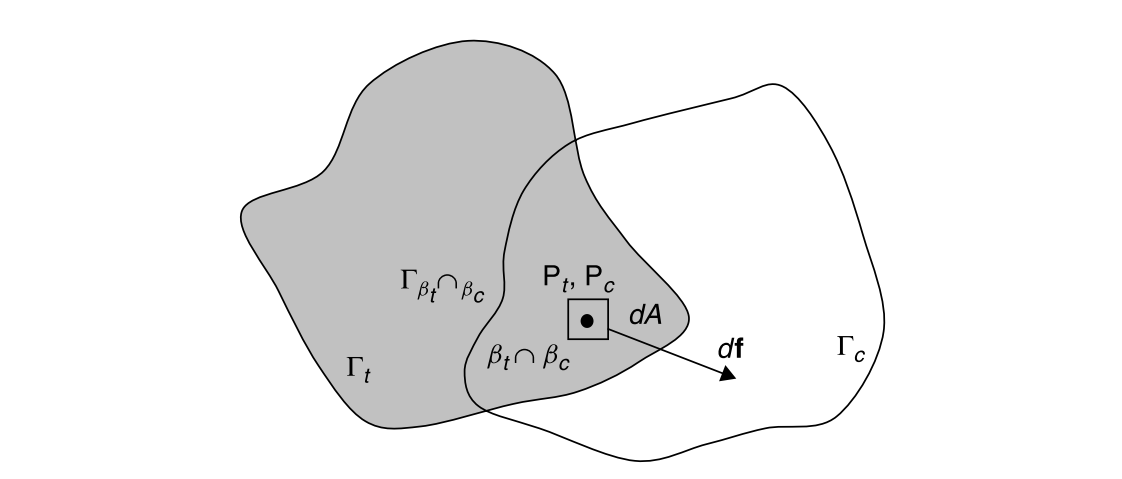
\includegraphics[width=\columnwidth]{Contact}
    \caption{Infinitesimal overlap of contractor and target body. \cite{Mun04}}
    \label{fig:contact}
\end{figure}

\bigbreak
The penetration distance $d$ for each case is given by \cite{Mun04}

\begin{equation}
    \label{eq:d}
    d=\frac{\sigma\,h}{p}\,,
\end{equation}

with applied pressure $\sigma$, element height $h$ and penalty factor $p$. 
\bigbreak
The penalty factor $p$ is given by

\begin{equation}
    \label{eq:p}
    p=\alpha\,E\,,
\end{equation}

with \rm{Young's Modulus} $E$ and a constant $\alpha$ (in this paper: $\alpha=10$) to regulate penetration. 

\bigbreak
Contact damping (Rayleigh damping, viscous damping) due to plastic deformation, breakage of surface asperities, etc. is given by \cite{Mun04}

\begin{equation}
    \label{eq:sigmac}
    \sigma_{\rm{C}}=4\,\xi\frac{\sqrt{p/\rho}}{h}\dot{d}\,,
\end{equation}

\addtocounter{footnote}{-1}
\stepcounter{footnote}
with damping ratio $0\leq\xi\footnotemark\leq1$ and finite element density $\rho$.  

\footnotetext{describes energy dissipation}

\bigbreak
The mass damping coefficient is given by

\begin{equation}
    \label{eq:massdamp}
    \zeta = \sqrt{E\,\rho}
\end{equation}